\section{Inventory} \label{InventoryScreen}

In this section the sketch of the inventory screen is going to be described. The functionality is going to be described as well as the design principles used in the design process. The sketch consists of 3 sketches of the screen, describing 3 different states of the inventory screen as can be seen in figure \ref{FinalInventorySketch}. The first screen from the left, shows the screen when no action has been taken. The second screen from the left shows an expanded ingredient. The third screen from the left shows the screen when the user is searching for an ingredient.

\begin{figure}[H]
    \centering
    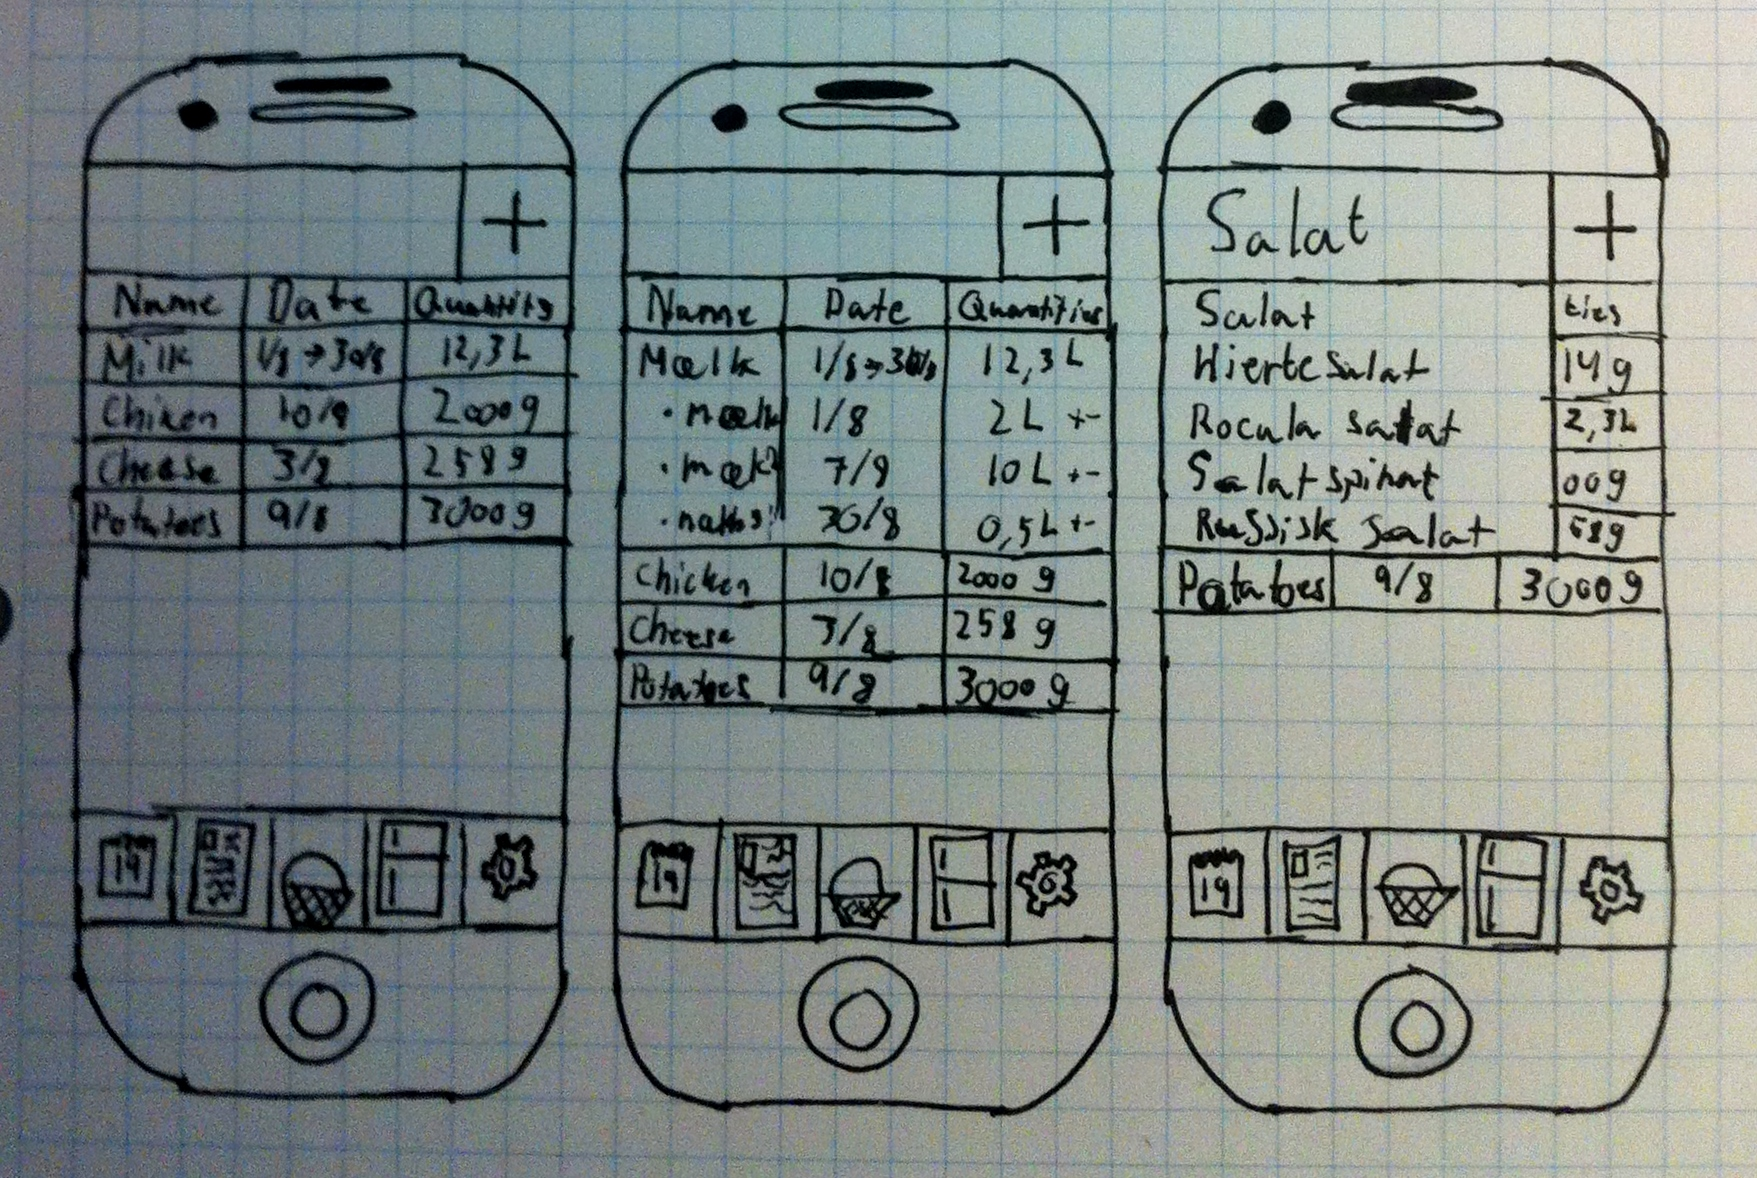
\includegraphics[width=0.5\textwidth]{Grafik/FoodPlanner/FinalInventorySketch}
    \caption{The final sketch of the inventory screens}
    \label{FinalInventorySketch}
\end{figure}

\subsection{Inventory overview screen}

The inventory overview screen is divided into two different elements, not taking the general design elements into consideration. These elements are:

\begin{itemize}
    \item Search bar
    \item Table
\end{itemize}

The search bar is placed in the top of the screen, as this is where a user most likely will look for it first, because on most mobile applications and also on websites, the search bar is located at the
top of the screen. The add icon is used to make the user able to add items to the inventory, that are not included in the ingredients of the meal plan.

The second element is the table, which is located under the search bar. The table is divided into three columns; name of the item, expiration date of the item, and the quantity of the item.

The first column with the name of the item only holds the information about the items name. The second column shows the expiration date of the item, if the user only have one instance of the item, meaning that there will only be one expiration date, only one expiration date is shown in the expiration date column, but if the user has more instances of an item and therefore different expirations dates, the first and the last expiration dates of the item will be shown, and an arrow in between the dates will indicate that the expiration dates go from the first to the last. The quantity column holds the information about the quantity of the item.

\subsection{Expanded ingredient list}

When the user click on an ingredient, the ingredient will expand and show all the instances of the information as shown on the second screen from the left in figure \ref{FinalInventorySketch}. The information is still stored in the three columns described in the inventory overview screen. An instance of the ingredient will therefore show the name of the instance, the expiration date and the quantity of the instance. 

\subsection{Searching for an ingredient}

The third screen from the left in figure \ref{FinalInventorySketch} shows the search function of the screen. When text is entered into the search box, the items in the search function will expand and lay over the ingredients in the inventory.

The search new overlay will show a fixed number of ingredients which has the searched text in their names, and the user can by clicking one of the ingredients, the expanded search bar will contract, and the item chosen will be shown in the search bar. By clicking the add icon the user will now be able to add the item to their inventory, and if the item already is in the inventory, the item will be an instance that the user can expand to see. The expiration date will then be changed in the table, as well with the quantity.